\section{Diagramas de colaboración} % (fold)
\label{sec:diagramas_de_colaboracion}

	Los diagramas de interacción son diagramas que describen cómo grupos de objetos colaboran para conseguir algún fin. Estos diagramas muestran objetos, así como los mensajes que se pasan entre ellos dentro del caso de uso, es decir, capturan el comportamiento de los casos de uso.
	
	Hay dos tipos de diagrama de interacción, ambos basados en la misma información, pero cada uno enfatizando un aspecto particular: Diagramas de Secuencia y \textbf{Diagramas de Colaboración.}

	Un diagrama de colaboración, se puede decir que es una forma alternativa al diagrama de secuencias a la hora de mostrar un escenario. \textbf{Este tipo de diagrama muestra las interacciones que ocurren entre los objetos que participan en una situación determinada.}

	\medskip
	
	\fcolorbox{negro}{gris}{\parbox{15cm}{El \textit{diagrama de colaboración} se enfoca en la relación entre los objetos y su topología de comunicación. En estos diagramas, los mensajes enviados de un objeto a otro se representan mediante flechas, acompañado del nombre del mensaje, los parámetros (si los tiene) y la secuencia del mensaje. Cada mensaje lleva un número de secuencia que denota cuál es el mensaje que le precede. La secuencia de los mensajes y los flujos de ejecución concurrentes deben determinarse explícitamente mediante números de secuencia.}}
	
	\medskip
		
	Estos diagramas están indicados para mostrar una situación o flujo de programa específico y son considerados uno de los mejores diagramas para mostrar o explicar rápidamente un proceso dentro de la lógica del programa.
	
	En este documento se detallan las principales colaboraciones relacionadas con todos los aspectos del proyecto. Por tanto, vamos a ver los diagramas de colaboración que hacen referencia a las \textit{Actividades Generales, las Actividades Específicas de los Médicos, las de los Pacientes, las del Administrador, y además, las colaboraciones relacionadas con las Fichas Médicas.}
	
	\subsection{Colaboraciones de las Actividades Generales} % (fold)
	\label{sub:colaboraciones_de_las_actividades_generales}
	
		En primer lugar veremos los diagramas de colaboraciones relacionados con las actividades generales, los cuales tienen correspondencia con los casos de uso vistos para esta misma sección.
		
		Las colaboraciones relacionadas con el registro de un nuevo usuario (en este caso de un paciente (Figura \ref{fig:col_reg_paciente})), en las que si todo es correcto, se crea una nueva instancia de usuario (en este caso de paciente), y por último, se informa de que todo es correcto. 
		
		En caso de error, por ejemplo, porque no se verifiquen los datos ó porque el usuario ya exista, lo que ocurre es que se informa del error al usuario y le redirige a la interfaz de registro(Figura \ref{fig:col_reg_paciente_err}).
		
		Esta forma de registrarse será la misma tanto para médicos como para pacientes. La diferencia son los datos que deben rellenar una vez que han accedido al sistema.
		
		\bigskip
		\bigskip
		
		\begin{figure}[H]
		  \centering
		    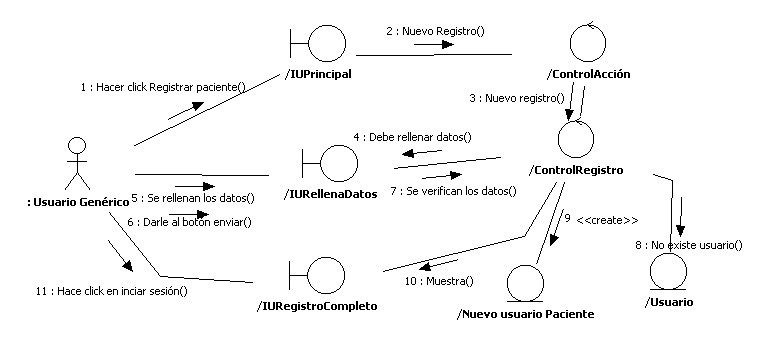
\includegraphics[width=16cm]{img/jpg/colaboraciones/17_Registrarse_paciente.jpg}
		  \caption{Registrarse como paciente}
		  \label{fig:col_reg_paciente}
		\end{figure}
	
		\begin{figure}[H]
		  \centering
		    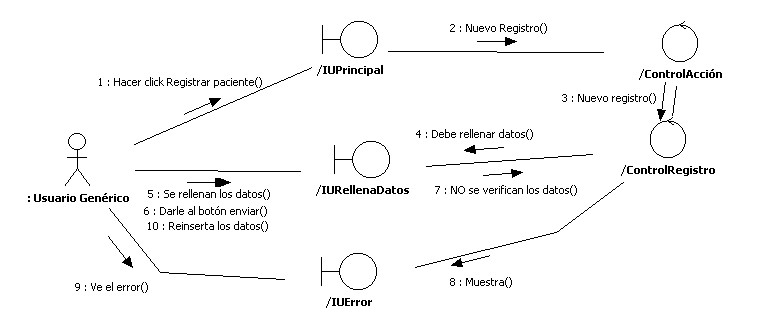
\includegraphics[width=16cm]{img/jpg/colaboraciones/18_RegistrarsePacienteError.jpg}
		  \caption{Error.- Registrarse como paciente}
		  \label{fig:col_reg_paciente_err}
		\end{figure}
		
		Una vez hemos realizado el registro, pasamos a las interfaces de rellenar datos. En función del rol de cada usuario, deberá rellenar unos datos u otros. Al finalizar, puede estar todo correcto (Figura \ref{fig:col_rellenarinfo}), o por el contrario puede aparecer algún error si no se verifica algún tipo de dato (Figura \ref{fig:col_rellenarinfo_err}).
		
		\begin{figure}[H]
		  \centering
		    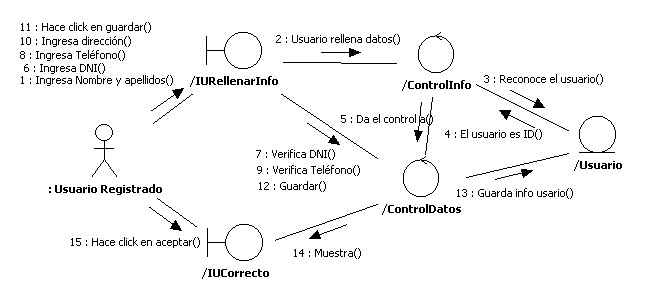
\includegraphics[width=16cm]{img/jpg/colaboraciones/19_RellenarInfo.jpg}
		  \caption{Rellenar información}
		  \label{fig:col_rellenarinfo}
		\end{figure}
		
		\begin{figure}[H]
		  \centering
		    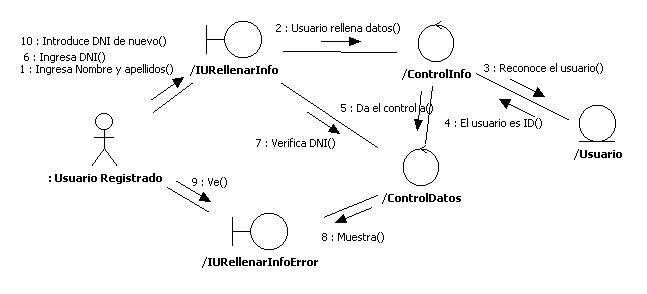
\includegraphics[width=16cm]{img/jpg/colaboraciones/20_RellenarInfoError.jpg}
		  \caption{Error.- Rellenar información}
		  \label{fig:col_rellenarinfo_err}
		\end{figure}
		
		Además, en el caso de ser médico, se debe rellenar información relativa a la consulta (Figura \ref{fig:col_rellenarinfo_consulta}), cómo puede ser la dirección, el teléfono de contacto, el precio, la especialidad, etcétera.
		
		\begin{figure}[H]
		  \centering
		    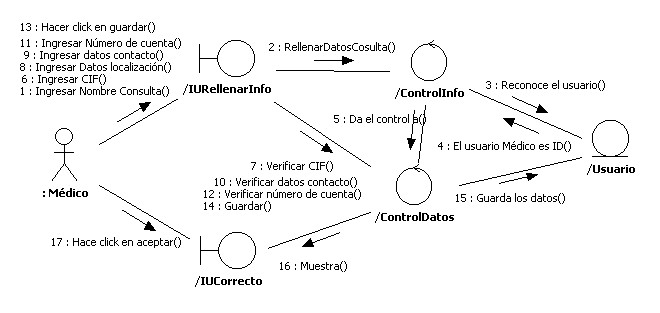
\includegraphics[width=16cm]{img/jpg/colaboraciones/21_RellenarInfoConsulta.jpg}
		  \caption{Rellenar información de la consulta}
		  \label{fig:col_rellenarinfo_consulta}
		\end{figure}
		
		\newpage
		Una vez que un usuario está registrado, podrá acceder a la aplicación (Figura \ref{fig:col_acc_y_aut}). Se identifica mediante el email y una contraseña. El sistema verifica que el usuario exista y que la contraseña sea correcta y se crea una nueva sesión y se accederá al \textit{dashboard}. Pueden aparecer errores, por ejemplo, si no existe el usuario, o si la contraseña introducida no es correcta. En dicho caso, se informará del error al usuario (Figura \ref{fig:col_acc_y_aut}).
		
		\begin{figure}[H]
		  \centering
		    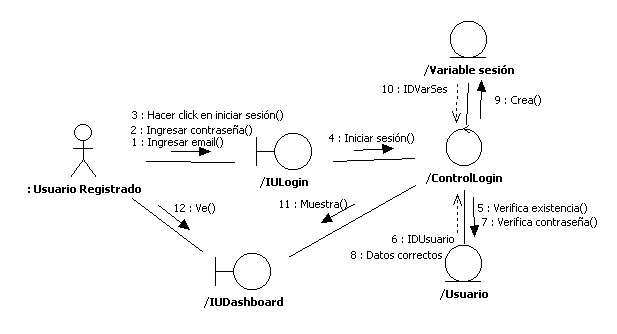
\includegraphics[width=16cm]{img/jpg/colaboraciones/23_Accesoyautentificacion.jpg}
		  \caption{Acceso y autentificación}
		  \label{fig:col_acc_y_aut}
		\end{figure}
		
		\begin{figure}[H]
		  \centering
		    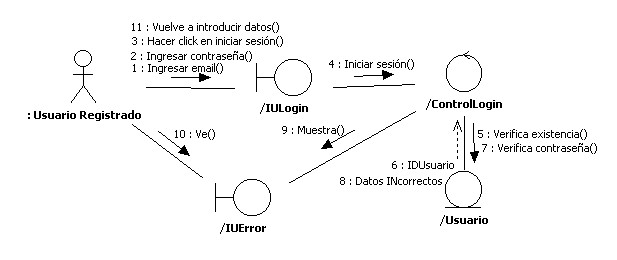
\includegraphics[width=16cm]{img/jpg/colaboraciones/24_AccesoyautentificacionError.jpg}
		  \caption{Error.- Acceso y autentificación}
		  \label{fig:col_acc_y_aut_err}
		\end{figure}
		
		Entre otras cosas, un usuario genérico podrá buscar cualquier médico antes de registrarte en el sistema para saber si le interesa (Figura \ref{fig:col_buscarmedico}). Si no encuentra ninguno, se notificará de que el médico no forma parte de la comunidad. Si lo encuentra, ofrece la posibilidad de ver su información.
		
		\begin{figure}[H]
		  \centering
		    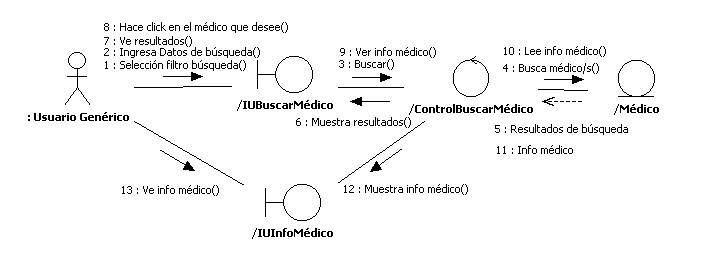
\includegraphics[width=16cm]{img/jpg/colaboraciones/22_BuscarMedico.jpg}
		  \caption{Buscar Médico}
		  \label{fig:col_buscarmedico}
		\end{figure}
		
		El resto de casos de uso relacionados con las \textit{Actividades Generales} son muy simples y son necesarios diagramas de colaboración.
		
	% subsection colaboraciones_de_las_actividades_generales (end)
	
	\newpage
	\subsection{Colaboraciones de los Médicos} % (fold)
	\label{sub:colaboraciones_de_los_medicos}
	
		En esta sección aparecen los principales diagramas de colaboraciones referentes a las actividades de los médicos.
		
		En primer lugar vemos que un médico debe realizar la configuración de sus datos. Si es la primera vez que accede al sistema, será lo primero con lo que se encuentre. En otro caso, siempre podrá acceder a los datos de su configuración en cualquier momento que lo desee. Si se produce algún cambio en la configuración, se almacenará dicho cambio en el \textit{historial del médico}. 
		
		Si la secuencia de acciones ha ocurrido correctamente, se mostrará un mensaje informando de que se ha actualizado la configuración con éxito (Figura \ref{fig:col_config_dat_medico}). Por el contrario, si se introduce algún tipo de datos incorrecto o con un formato no adecuado se producirá un error (Figura \ref{fig:col_config_dat_medico_err}). También pueden existir errores en el caso de que todos los datos introducidos sean en principio correctos, pero no se puedan almacenar o guardar en el usuario correspondiente (Figura \ref{fig:col_config_dat_medico_err2}).
		%\begin{landscape}
		\bigskip
		
		\begin{figure}[H]
		  \centering
		    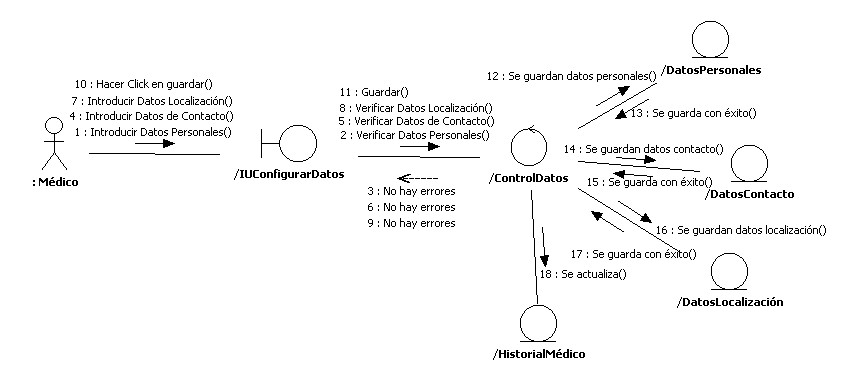
\includegraphics[width=16cm]{img/jpg/colaboraciones/1_ConfiguracionDatosMedico.jpg}
		  \caption{Configuración de los datos del médico}
		  \label{fig:col_config_dat_medico}
		\end{figure}
		
		\bigskip
		\bigskip
		\bigskip
		\begin{figure}[H]
		  \centering
		    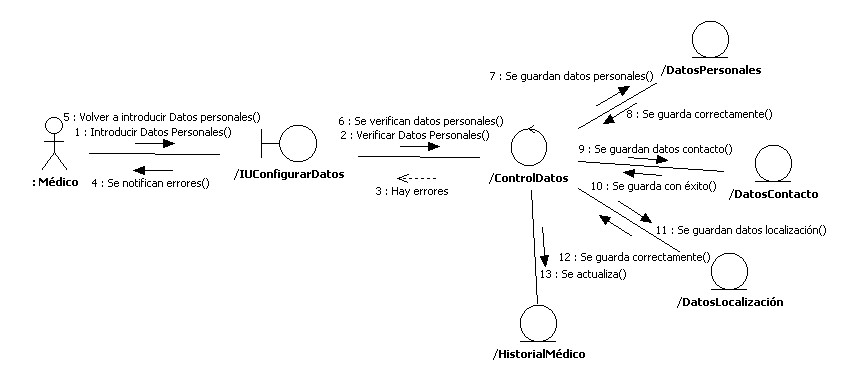
\includegraphics[width=16cm]{img/jpg/colaboraciones/2_ConfiguracionDatosMedicoError1.jpg}
		  \caption{Error.- Configuración de los datos del médico}
		  \label{fig:col_config_dat_medico_err}
		\end{figure}
		
		\bigskip
		\bigskip
		\bigskip
		\begin{figure}[H]
		  \centering
		    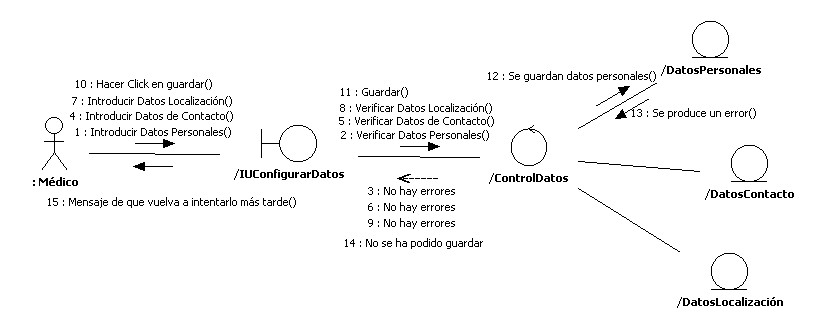
\includegraphics[width=16cm]{img/jpg/colaboraciones/3_ConfiguracionDatosMedicoError2.jpg}
		  \caption{Error.- Configuración de los datos del médico}
		  \label{fig:col_config_dat_medico_err2}
		\end{figure}
		
		\newpage
		
		Además de poder modificar su información personal, un médico puede realizar cambios en los datos de su cuenta, como son, por ejemplo, el email, nombre de usuario o la contraseña (Figura \ref{fig:col_config_cuenta_medico}). Si no existe ningún error (Figura \ref{fig:col_config_cuenta_medico_err}), se guardarán los cambios, se actualizará el \textit{historial del médico} y se informará de que todo ha ido correctamente. En caso contrario, se notificará al usuario el motivo del error y que sus cambios no han sido realizados.
		\begin{figure}[H]
		  \centering
		    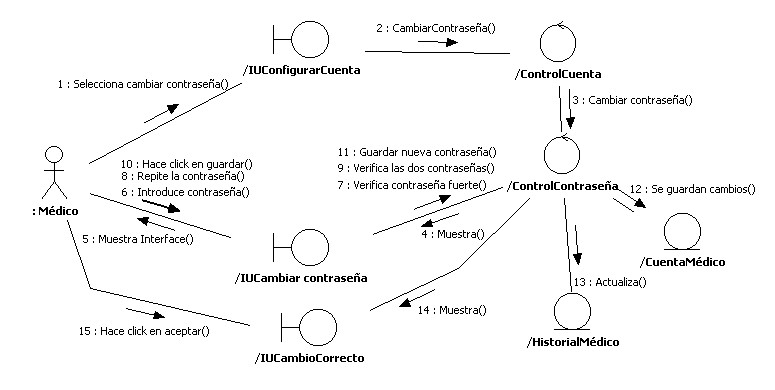
\includegraphics[width=16cm]{img/jpg/colaboraciones/4_ConfiguracionCuentaMedico.jpg}
		  \caption{Configuración de la cuenta del médico}
		  \label{fig:col_config_cuenta_medico}
		\end{figure}
		
		\begin{figure}[H]
		  \centering
		    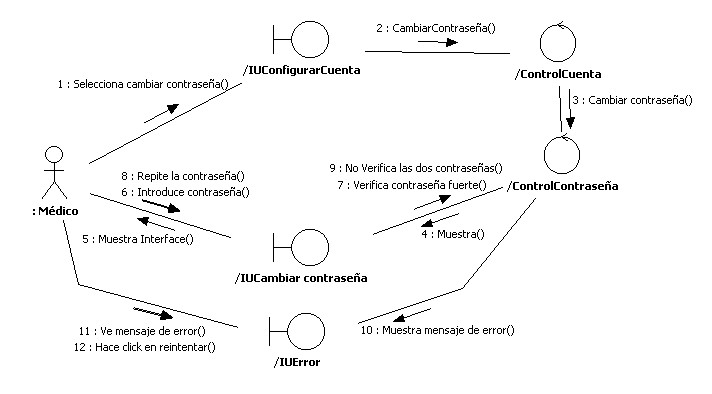
\includegraphics[height=7cm, width=16cm]{img/jpg/colaboraciones/5_ConfiguracionCuentaMedicoError.jpg}
		  \caption{Error.- Configuración de la cuenta del médico}
		  \label{fig:col_config_cuenta_medico_err}
		\end{figure}
		
		Uno de los aspectos fundamentales que debe configurar un médico es su horario, introduciendo principalmente \textit{cuales son sus días laborales, el rango de horas de su jornada laboral o su precio medio}. Podrá modificar esta información en cualquier momento que lo desee. Si la secuencia de acciones es validada y, por tanto, correcta, se guardarán los cambios en su horario, se actualizará el \textit{historial del médico} y se notificará (Figura \ref{fig:col_config_horario_medico}). Por el contrario, si algún dato no se verifica o si no se puede guardar la información en ese momento por cualquier motivo, se mostrará un mensaje notificando dicho fallo (Figura \ref{fig:col_config_horario_medico_err}).
		
		\begin{figure}[H]
		  \centering
		    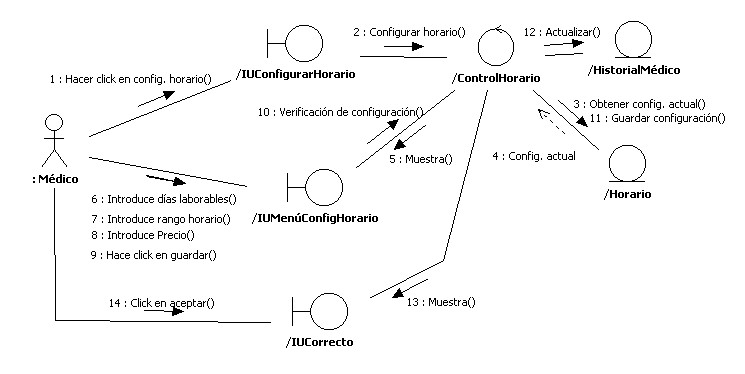
\includegraphics[width=16cm, height=7cm]{img/jpg/colaboraciones/6_ConfiguracionHorarioMedico.jpg}
		  \caption{Configuración del horario del médico}
		  \label{fig:col_config_horario_medico}
		\end{figure}
		
		\begin{figure}[H]
		  \centering
		    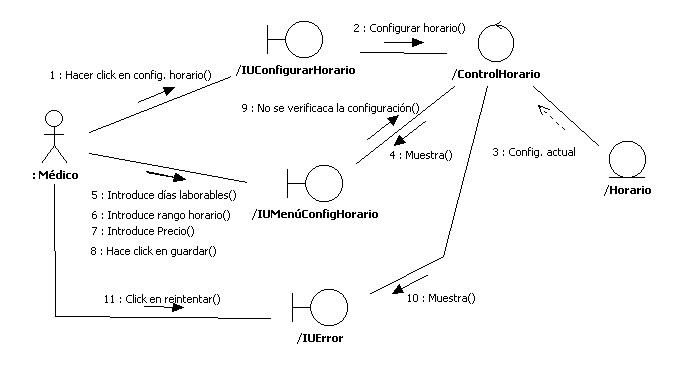
\includegraphics[width=16cm, height=7cm]{img/jpg/colaboraciones/7_ConfiguracionHorarioMedicoError.jpg}
		  \caption{Error.- Configuración del horario del médico}
		  \label{fig:col_config_horario_medico_err}
		\end{figure}
		
		El médico podrá ver un horario en vista semanal con las citas que tiene asignadas (Figura \ref{fig:col_vistasemanal_medico}). Además, desde dicha vista podrá ver la ficha médica de sus pacientes (Figura \ref{fig:col_verficha_medico}) y anular una cita puntual (Figura \ref{fig:col_anular_medico}).
		
		\begin{figure}[H]
		  \centering
		    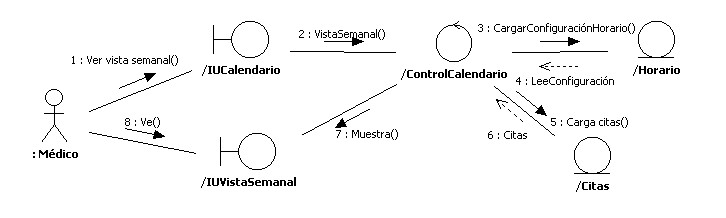
\includegraphics[width=16cm]{img/jpg/colaboraciones/8_VistaSemanalMedico.jpg}
		  \caption{Vista semanal del médico}
		  \label{fig:col_vistasemanal_medico}
		\end{figure}
		
		Anular una cita puntual (Figura \ref{fig:col_anular_medico}) requiere confirmación. Además, puede escribir el mensaje que le llegará al afectado. Quedará registrado en el \textit{historial del médico y en el del paciente}.
		\begin{figure}[H]
		  \centering
		    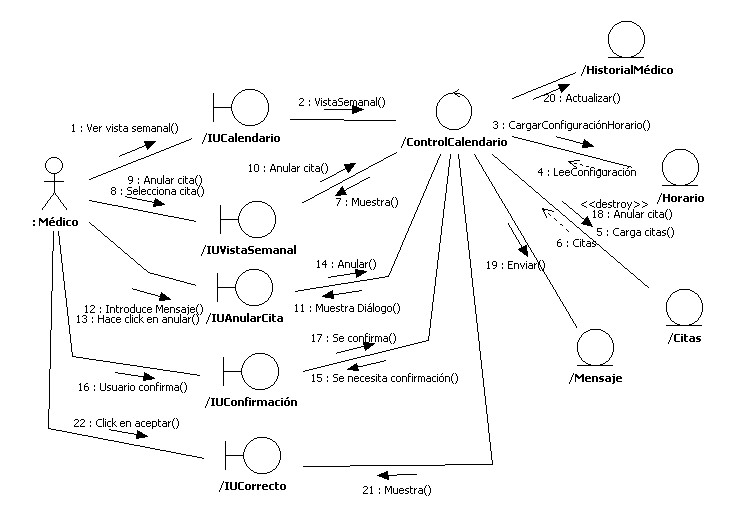
\includegraphics[width=16cm, height=10.5cm]{img/jpg/colaboraciones/9_AnularCitaMedico.jpg}
		  \caption{El médico anula una cita}
		  \label{fig:col_anular_medico}
		\end{figure}
		
		A la hora de anular una cita (Figura \ref{fig:col_anular_medico}), un médico siempre podrá retractarse y cancelar la acción (Figura \ref{fig:col_cancelaranular_medico}). Por eso, entre otras cosas, debe existir confirmación.
		
		\begin{figure}[H]
		  \centering
		    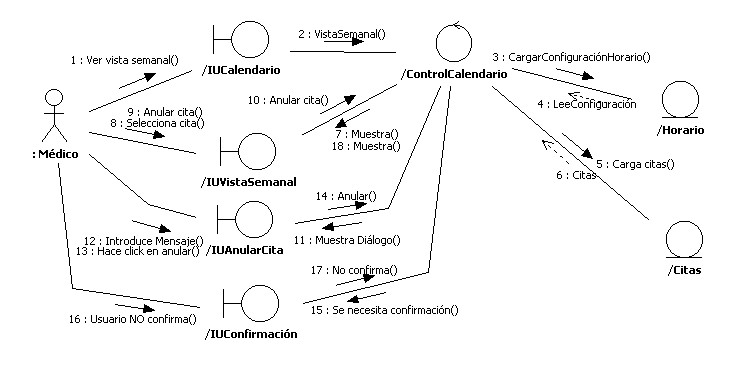
\includegraphics[width=16cm]{img/jpg/colaboraciones/10_AnularCitaMedicoCancelar.jpg}
		  \caption{El médico cancela anular una cita}
		  \label{fig:col_cancelaranular_medico}
		\end{figure}
		
		Un médico, además, podrá ver la ficha médica de un paciente (Figura \ref{fig:col_verficha_medico}). Ésta acción podrá realizarla tanto después de realizar una búsqueda de uno de sus pacientes como desde el calendario. Puede ir todo correcto, o por el contrario aparecer algún error inusual (Figura \ref{fig:col_verficha_medico_err}).
		
		\begin{figure}[H]
		  \centering
		    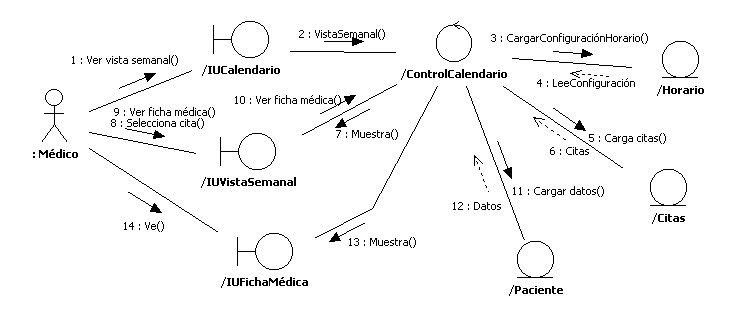
\includegraphics[width=16cm]{img/jpg/colaboraciones/11_VerFichaMedica.jpg}
		  \caption{El médico ve una ficha médica}
		  \label{fig:col_verficha_medico}
		\end{figure}
		
		\begin{figure}[H]
		  \centering
		    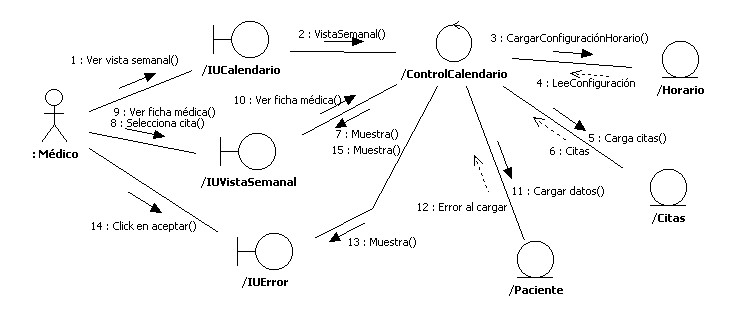
\includegraphics[width=16cm]{img/jpg/colaboraciones/12_VerFichaMedicaError.jpg}
		  \caption{Error.- Médico viendo una ficha médica}
		  \label{fig:col_verficha_medico_err}
		\end{figure}
		
		Otra de las acciones que puede realizar un usuario con rol de médico es ver la lista de todos sus pacientes (Figura \ref{fig:col_ver_pacientes_medico}). Puede que en dicho momento ocurra un error de acceso, el cuál será notificado inmediatamente (Figura \ref{fig:col_ver_pacientes_medico_err}).
		
		\begin{figure}[H]
		  \centering
		    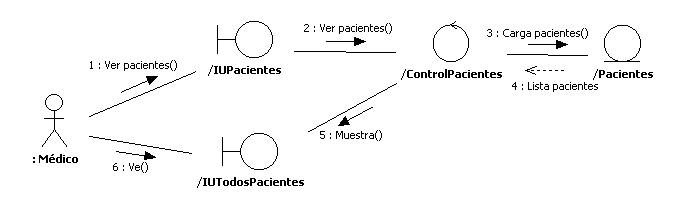
\includegraphics[width=16cm]{img/jpg/colaboraciones/13_VerTodosPacientes.jpg}
		  \caption{El médico ve la lista de sus pacientes}
		  \label{fig:col_ver_pacientes_medico}
		\end{figure}
		
		\begin{figure}[H]
		  \centering
		    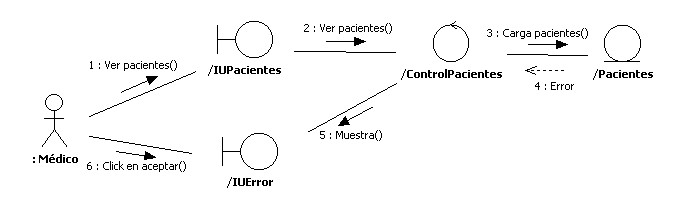
\includegraphics[width=16cm]{img/jpg/colaboraciones/14_VerTodosPacientesError.jpg}
		  \caption{Error.- El médico ve la lista de sus pacientes}
		  \label{fig:col_ver_pacientes_medico_err}
		\end{figure}
		
		La última de las principales acciones será la de buscar un paciente concreto (Figura \ref{fig:col_buscarpaciente_medico}). Ésta acción se puede llevar a cabo mediante distintos tipos de búsqueda. Si no encuentra ningún paciente, o si se produce algún error, se notificará mediante la interfaz (Figura \ref{fig:col_buscarpaciente_medico_err}).
		
		\begin{figure}[H]
		  \centering
		    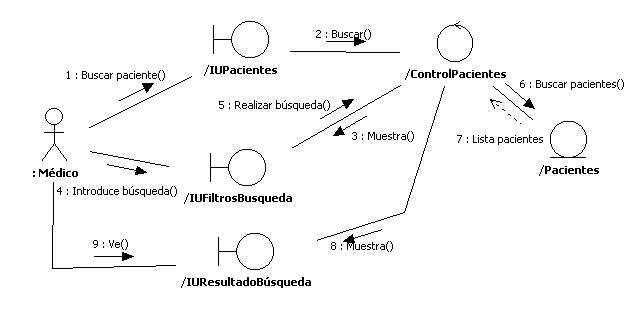
\includegraphics[width=16cm]{img/jpg/colaboraciones/15_BuscarPaciente.jpg}
		  \caption{Buscar Paciente}
		  \label{fig:col_buscarpaciente_medico}
		\end{figure}
		
		\begin{figure}[H]
		  \centering
		    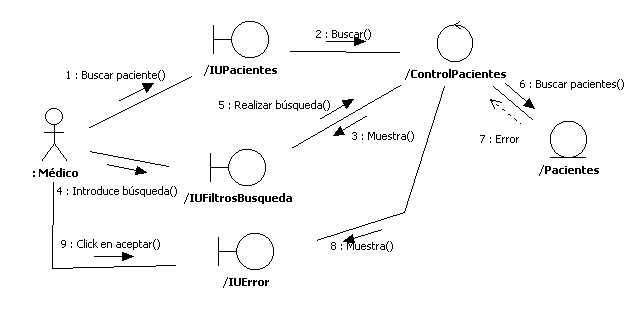
\includegraphics[width=16cm]{img/jpg/colaboraciones/16_BuscarPacienteError.jpg}
		  \caption{Error.- Buscar paciente}
		  \label{fig:col_buscarpaciente_medico_err}
		\end{figure}
		
	% subsection colaboraciones_de_los_médicos (end)
	
	\newpage
	\subsection{Colaboraciones de los Pacientes} % (fold)
	\label{sub:colaboraciones_de_los_pacientes}
				
		Los diagramas de colaboraciones relacionados con la configuración de la información personal y de los datos de la cuenta del usuario con rol paciente, son prácticamente los mismos que los ya vistos para los usuarios con rol de médico. Las pequeñas diferencias son que las entidades serán los pacientes (en lugar de médicos), y que se modificará el \textit{historial del paciente (en lugar de el historial del médico)}.
		
		Por su parte, un paciente también podrá ver una vista semanal de su calendario, con las citas que tiene previstas (Figura \ref{fig:col_vistasemanal_paciente}). Desde ella podrá ver la información del médico (Figura \ref{fig:col_verinfo_medico_paciente}) y anular una cita (Figura \ref{fig:col_anulacita_paciente}).
		
		\bigskip
		\bigskip
		\begin{figure}[H]
		  \centering
		    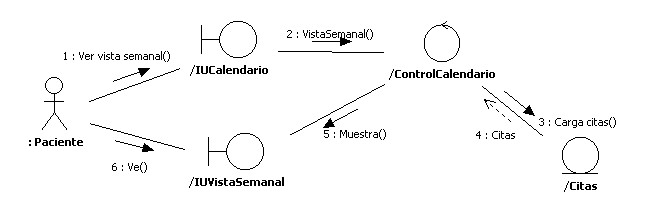
\includegraphics[width=16cm]{img/jpg/colaboraciones/25_VistaSemanalPaciente.jpg}
		  \caption{Vista semanal del paciente}
		  \label{fig:col_vistasemanal_paciente}
		\end{figure}
		
		\bigskip
		\bigskip
		
		Cuando un paciente anula una cita, debe tener en cuenta que sea antes de la fecha y hora concebida para poder hacerlo sin recibir ningún recargo. 
		
		Esta acción siempre requiere confirmación por parte del usuario. Si llega a anularse, se guardará el registro de lo ocurrido en el \textit{historial del médico y en el historial del paciente}. Una vez anulado, se notificará mediante la interfaz (Figura \ref{fig:col_anulacita_paciente}). Además, tanto al médico como al paciente les llegará un email informando de que la cita ha sido cancelada (en el caso de que así lo tengan configurado).
		
		Por otro lado, una vez hemos entrado en el camino de anular una cita, siempre tendremos la posibilidad de cancelar la acción, o bien de no confirmarla (Figura \ref{fig:col_anularcita_paciente_cancelar}).
		
		Podemos ver que es un diagrama de colaboración bastante similar al de anular cita de un médico (Figura \ref{fig:col_anular_medico}).
		
		\begin{figure}[H]
		  \centering
		    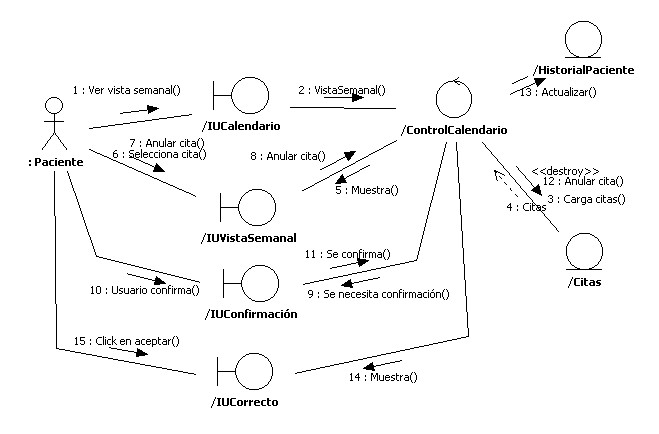
\includegraphics[width=16cm]{img/jpg/colaboraciones/26_AnularCitaPaciente.jpg}
		  \caption{El paciente anula una cita}
		  \label{fig:col_anulacita_paciente}
		\end{figure}
		
		\begin{figure}[H]
		  \centering
		    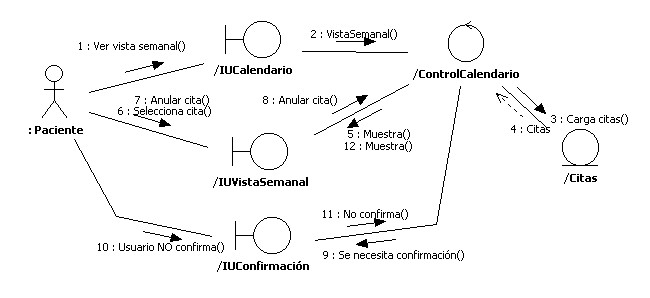
\includegraphics[width=16cm]{img/jpg/colaboraciones/27_AnularCitaPacienteCancelar.jpg}
		  \caption{El paciente cancela anular una cita}
		  \label{fig:col_anularcita_paciente_cancelar}
		\end{figure}
		
		Tanto desde la vista semanal, cómo si se ha realizado una búsqueda, un paciente podrá ver la información de un médico (Figura \ref{fig:col_verinfo_medico_paciente}). Si no se produce ningún error, se mostrará la información. En caso contrario, se notificará mediante la interfaz. Además, esta acción también puede ser usada por un usuario genérico tras buscar un médico desde el \textit{Home} de la página web.
		
		\begin{figure}[H]
		  \centering
		    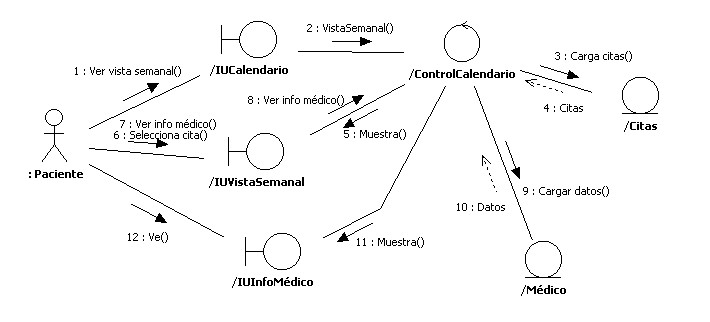
\includegraphics[width=16cm]{img/jpg/colaboraciones/28_VerInfoMedico.jpg}
		  \caption{Ver información de un médico}
		  \label{fig:col_verinfo_medico_paciente}
		\end{figure}
		
		Un paciente, además, podrá realizar búsquedas de médicos en función de diversos filtros (Figura \ref{fig:col_buscarmedico_paciente}). En el caso de no encontrar resultados o de que exista algún error, se informará al usuario.
		
		\begin{figure}[H]
		  \centering
		    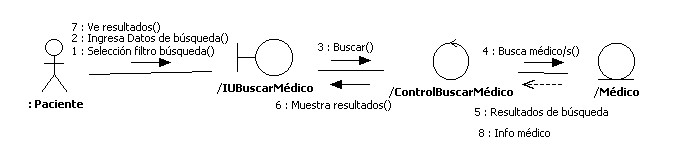
\includegraphics[width=16cm]{img/jpg/colaboraciones/29_PacienteBuscarMedico.jpg}
		  \caption{El paciente busca un médico}
		  \label{fig:col_buscarmedico_paciente}
		\end{figure}
		
		\bigskip
		\bigskip
		Una vez hemos realizada la búsqueda de un médico, podremos ver su horario, y además, asignarnos una cita. La vista del horario nos proporcionará gráficamente las horas libres de las que dispone el médico (Figura \ref{fig:col_verhorario_paciente}). En caso de querer asignarnos una cita (Figura \ref{fig:col_asigcita_paciente}), seleccionaremos la que más nos convenga. Si todo ocurrió correctamente, se guardará un registro en el \textit{historial del médico y en el del paciente} y se enviarán las correspondiente notificaciones vía email (si así lo tienen configurado).
		
		\begin{figure}[H]
		  \centering
		    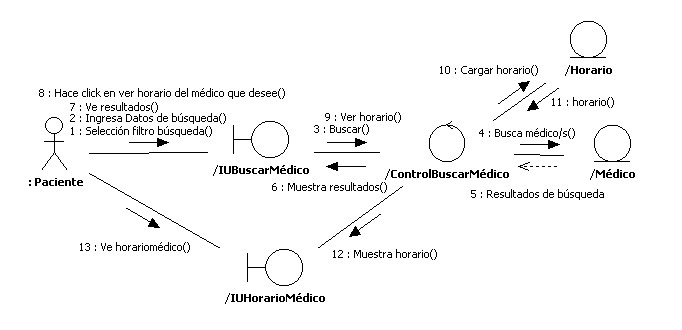
\includegraphics[width=16cm]{img/jpg/colaboraciones/30_VerhoarioMedico.jpg}
		  \caption{Ver el horario de un médico}
		  \label{fig:col_verhorario_paciente}
		\end{figure}
		
		\begin{figure}[H]
		  \centering
		    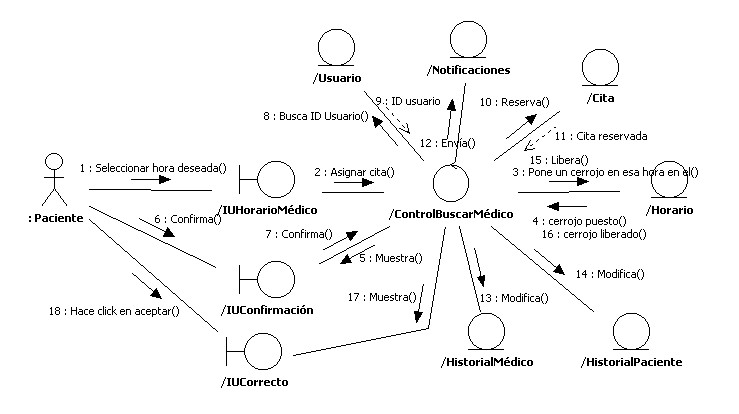
\includegraphics[width=16cm]{img/jpg/colaboraciones/31_AsignarseCita.jpg}
		  \caption{Asignarse una cita}
		  \label{fig:col_asigcita_paciente}
		\end{figure}
		
		
	% subsection colaboraciones_de_los_pacientes (end)

	\newpage
	\subsection{Colaboraciones de las Fichas Médicas} % (fold)
	\label{sub:colaboraciones_de_las_fichas_medicas}
	
		Hay una serie de actividades relacionadas con las fichas médicas que pueden realizar tanto médicos como pacientes. Todas ellas son bastante similares.
		
		En primer lugar tenemos las colaboraciones relacionadas con los antecedentes (pueden ser fisiológicos, familiares y personales). Vamos a representar sólo los fisiológicos, siendo el resto muy similares.
		
		Podremos ver una lista con los antecedentes (Figura \ref{fig:col_ant_fis_fm}), así como también añadir nuevos (\ref{fig:col_ant_fis_fm_anadir}) o modificar los existentes (Figura \ref{fig:col_ant_fis_fm_modificar}).
		
		\bigskip
		\bigskip
		\begin{figure}[H]
		  \centering
		    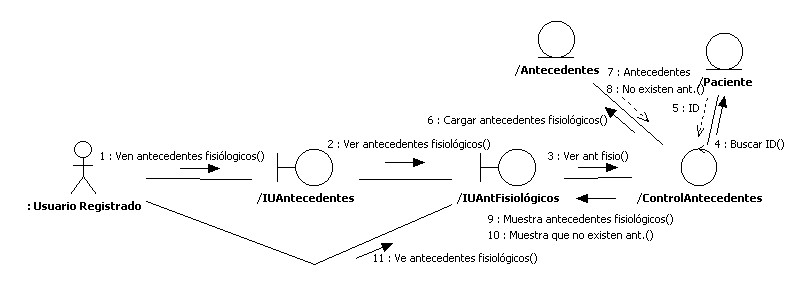
\includegraphics[width=16cm]{img/jpg/colaboraciones/32_VerAntecedentesFisiologicos.jpg}
		  \caption{Ver los antecedentes fisiológicos}
		  \label{fig:col_ant_fis_fm}
		\end{figure}
		
		\bigskip
		En el caso de añadir antecedentes (Figura \ref{fig:col_ant_fis_fm_anadir}), debemos tener en cuenta de que tipo son (en este diagrama son fisiológicos), y asegurarnos del paciente al que pertenecen. Una vez hecho esto, se creará el antecedente, se nos mostrará una nueva interfaz en la que deberemos rellenar los datos correspondientes, los cuales deben ser verificados por la unidad de control antes de guardarse y actualizarse. Si el antecedente se crea y se guarda correctamente, se informará al usuario y se mostrará la lista de los antecedentes. Además, se modificará el \textit{historial de la ficha médica}.
		
		Si existiese algún error (Figura \ref{fig:col_ant_fis_fm_anadir_err}) a la hora de crear el antecedente o de introducir la información, se notificaría al usuario.
		
		A la hora de realizar modificaciones en algún antecedente (Figura \ref{fig:col_ant_fis_fm_modificar}), el proceso es muy similar al de \textit{añadirlos}. En este caso, deberemos seleccionar un antecedente de los que ya existen, y a partir de ahí deberemos modificar los datos en la interfaz correspondiente. Si los datos introducidos son correctos y se actualiza correctamente, se mostrará un mensaje informando de que el proceso ha salido bien y se volverá a mostrar la lista de antecedentes. Si aparece algún error, se notificará al usuario (Figura \ref{fig:col_ant_fis_fm_modificar_err})
		
		\bigskip
		\bigskip
		\begin{figure}[H]
		  \centering
		    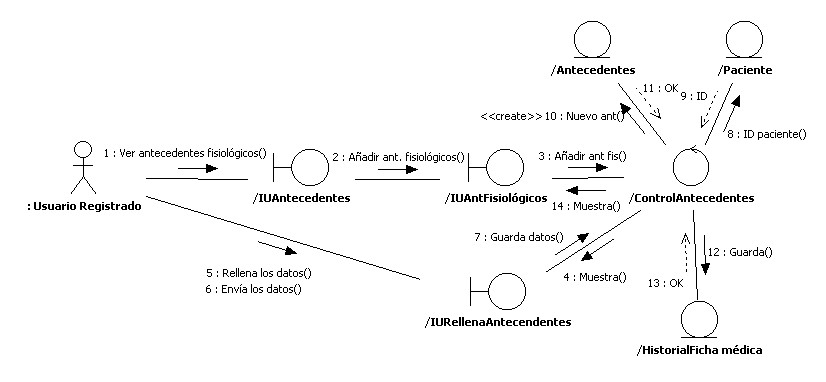
\includegraphics[width=16cm]{img/jpg/colaboraciones/33_AnadirAntecedente.jpg}
		  \caption{Añadir antecedentes fisiológicos}
		  \label{fig:col_ant_fis_fm_anadir}
		\end{figure}
		
		\bigskip
		\bigskip
		\begin{figure}[H]
		  \centering
		    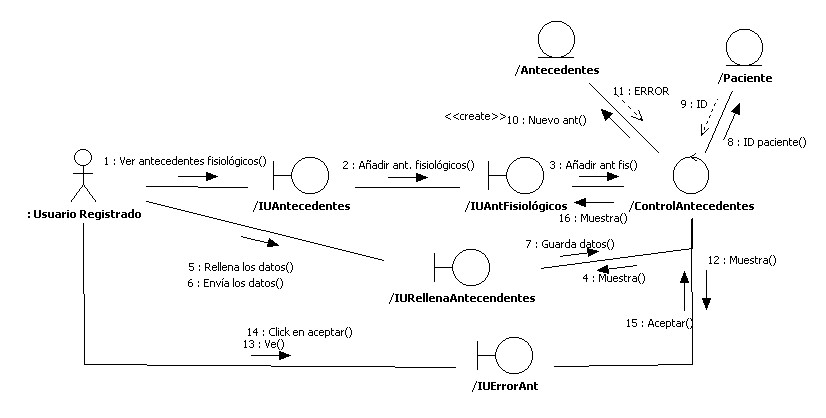
\includegraphics[width=16cm]{img/jpg/colaboraciones/34_AnadirAntecedenteError.jpg}
		  \caption{Error.- Añadir antecedentes fisiológicos}
		  \label{fig:col_ant_fis_fm_anadir_err}
		\end{figure}
		
		\begin{figure}[H]
		  \centering
		    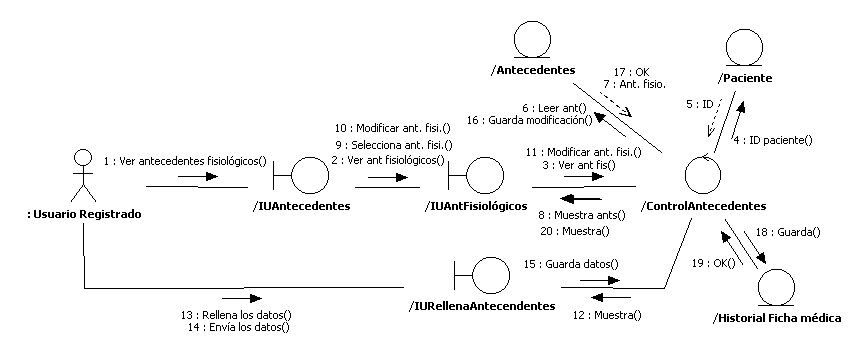
\includegraphics[width=16cm]{img/jpg/colaboraciones/35_ModificarAntecedente.jpg}
		  \caption{Modificar antecedentes fisiológicos}
		  \label{fig:col_ant_fis_fm_modificar}
		\end{figure}
		
		\begin{figure}[H]
		  \centering
		    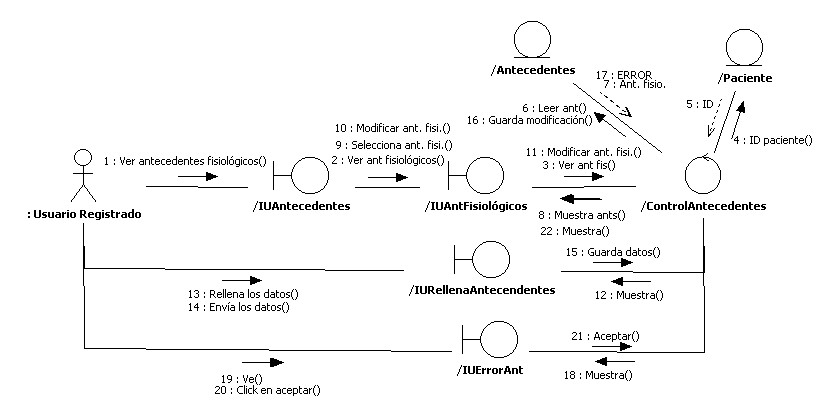
\includegraphics[width=16cm]{img/jpg/colaboraciones/36_ModificarAntecedenteError.jpg}
		  \caption{Error.- Modificar antecedentes fisiológicos}
		  \label{fig:col_ant_fis_fm_modificar_err}
		\end{figure}
		
		
		\newpage
		Con los diagnósticos, así como con el resto de posibles tipos de pruebas, los diagramas de colaboraciones son muy similares, cambiando principalmente la entidad (antecedente, diagnóstico, etcétera) en función de su tipo. Encontraremos la posibilidad de ver, añadir y modificar diagnósticos, tratamientos, observaciones, pruebas varias, etcétera.
		
		A continuación se muestran las colaboraciones relacionadas con los diagnósticos.
		\begin{figure}[H]
		  \centering
		    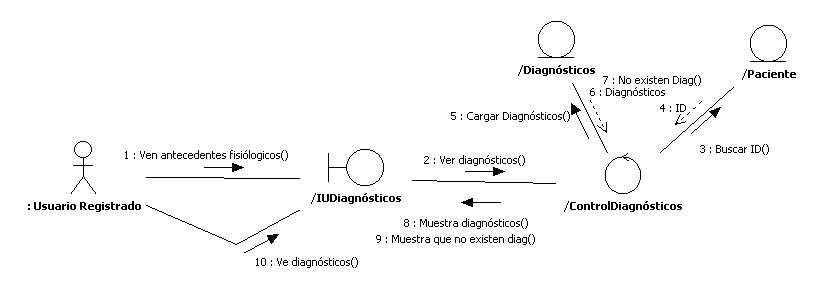
\includegraphics[width=16cm]{img/jpg/colaboraciones/37_VerDiagnosticos.jpg}
		  \caption{Ver diagnósticos}
		  \label{fig:col_diag_fm}
		\end{figure}
		
		\begin{figure}[H]
		  \centering
		    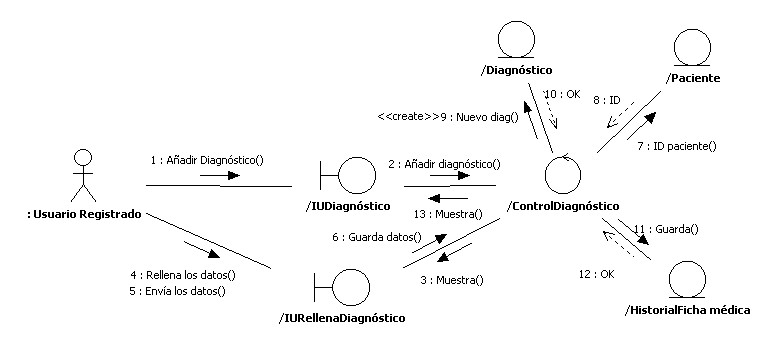
\includegraphics[width=16cm]{img/jpg/colaboraciones/38_AnadirDiagnostico.jpg}
		  \caption{Añadir diagnósticos}
		  \label{fig:col_diag_fm_anadir}
		\end{figure}
		
		\begin{figure}[H]
		  \centering
		    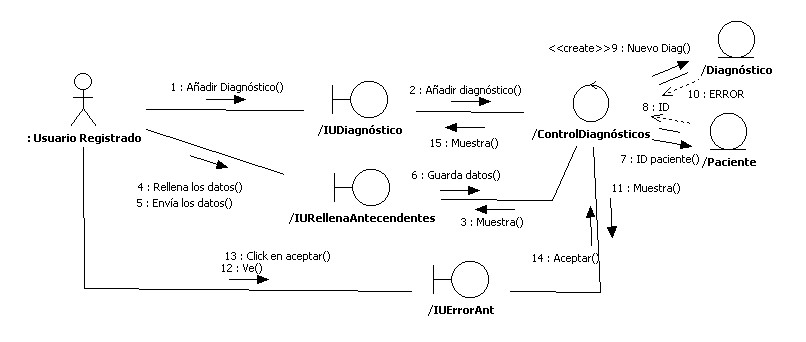
\includegraphics[width=16cm]{img/jpg/colaboraciones/39_AnadirDiagnosticoError.jpg}
		  \caption{Error.- Añadir diagnósticos}
		  \label{fig:col_diag_fm_anadir_err}
		\end{figure}
		
		\begin{figure}[H]
		  \centering
		    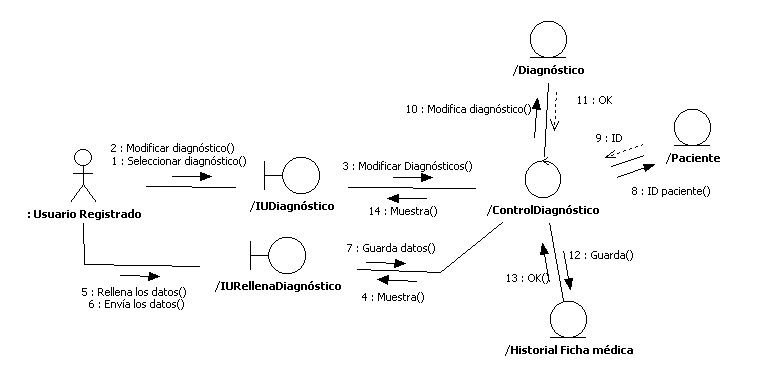
\includegraphics[width=16cm]{img/jpg/colaboraciones/40_ModificarDiagnostico.jpg}
		  \caption{Modificar diagnósticos}
		  \label{fig:col_diag_fm_modificar}
		\end{figure}
		
		\begin{figure}[H]
		  \centering
		    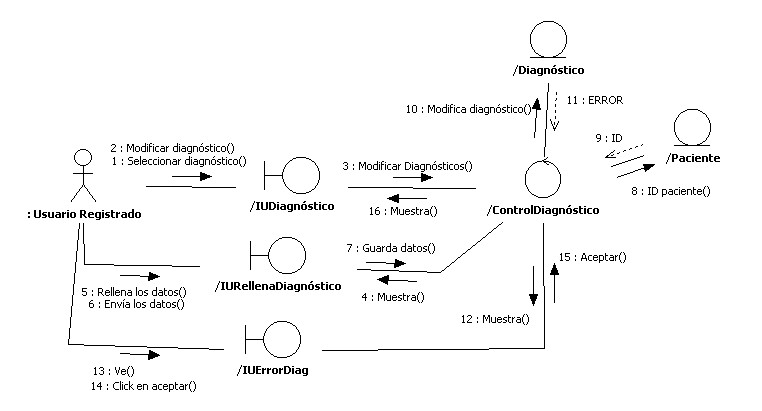
\includegraphics[width=16cm]{img/jpg/colaboraciones/41_ModificarDiagnosticoError.jpg}
		  \caption{Error.- Modificar diagnósticos}
		  \label{fig:col_diag_fm_modificar_error}
		\end{figure}
		
	% subsection colaboraciones_de_las_fichas_médicas (end)

	\newpage
	\subsection{Colaboraciones del Administrador} % (fold)
	\label{sub:colaboraciones_del_administrador}
	
		El principal diagrama de colaboración que debemos ver en esta sección es el de verificar médico. Una vez verificado, se hará visible para el resto de usuarios y se le notificará de que su cuenta está activa.
		
		\begin{figure}[H]
		  \centering
		    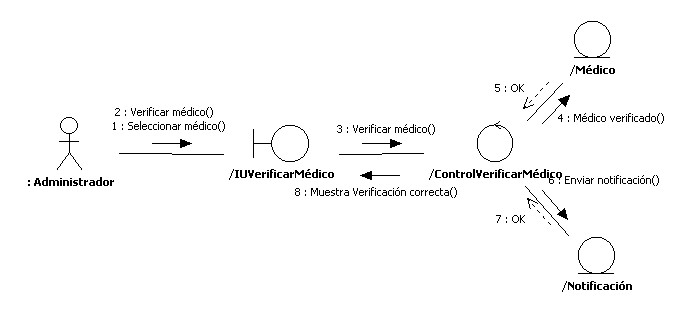
\includegraphics[width=16cm]{img/jpg/colaboraciones/42_VerificarMedico.jpg}
		  \caption{Verificar médico}
		  \label{fig:col_verificar_admin}
		\end{figure}
	
	% subsection colaboraciones_del_administrador (end)
	
% section diagrama_de_lolaboraciones (end)

